Presence of presence of non-specific fluorescence lighting, which is the fluorescence lightning produced by other cell parts that were not target in the staining procedures, can be troublesome for organelles like Golgi (see Figure \ref{fig:golgi-enhancement}). In order to mitigate this proble background removal algorithm described in this section can be used.

The rolling ball algorithm was introduced by \cite{Sternberg_1983} and is still widely used for processing medical and biological data. The idea of this algorithm is based on morphological opening of the image. 

\begin{definition}[Morphological opening]
	\label{def:morphological-opening}
	Morphological opening is an operation in image processing, when an image is first eroded and then dilated using the same structuring element. 
\end{definition}

Morphological opening is helpful for removing noisy elements, thin lines, while preserving bigger objects in the image (\cite{morph_open}).

A structuring element is an analog of a kernel in image processing. It is a matrix of zeros and ones (true and false), where ones represent the elements that will be used to perform the morphological operation and others will be ignored (see an example in Figure \ref{fig:rolling-ball} [left]). Such a structuring element is applied across the whole input image producing a new image based on the rules of a morphological operation it performs.  

For example, morphological dilation takes a new value of the pixel as the maximum value of its neighbors within the structuring element. Therefore, after this operation, the lines will be thicker and in general objects will appear bigger.

Whereas morphological erosion turns the pixel value into the minimum value of its neighbors within the structuring element. After this operation the floating pixels will be removed and all objects become smaller and thinner.

\cite{Sternberg_1983} has extrapolated the operation of morphological opening from 2D into 3D space. He defines a new interpretation of a 2D image in a 3D world called umbra. Umbra can be described as a 3D plane, where the height of each point is determined by its intesity value.

The structuring element for morphological opening of an umbra has to be then also a 3D object --- in this case a ball. Morphological opening of an umbra is a union of translations of the 3D structuring element that can be entirely contained inside it (see Figure \ref{fig:rolling-ball}). One can imagine the ball freely moving inside the volume constrained by the upper surface of an umbra. The opening then consists of all the pixels that can be reached by the ball. The radius of the ball is a hyper-parameter which has to be tuned.

\begin{figure}[H]
    \centering
    \subfloat[Structuring element]{{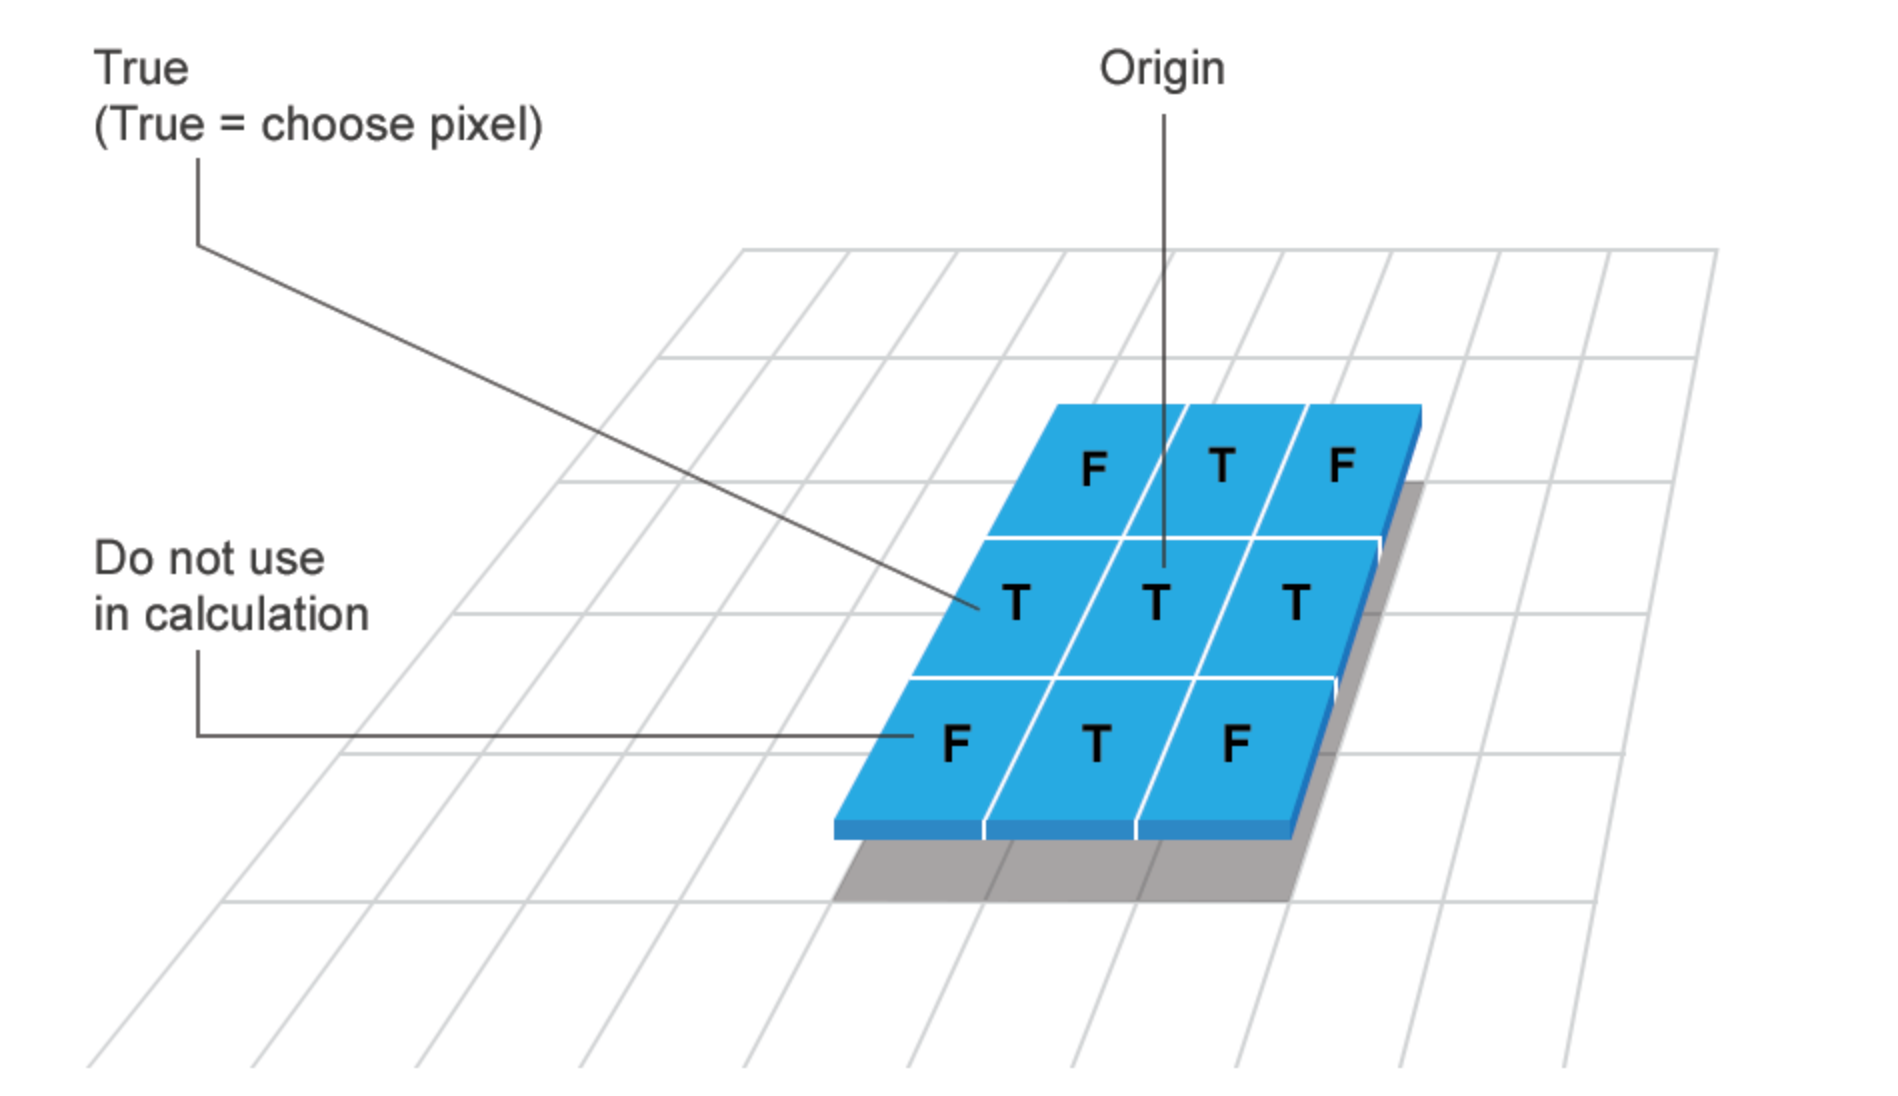
\includegraphics[width=0.3\linewidth]{bilder/structuring-element.png} }}
    \qquad
    \subfloat[Rolling ball]{{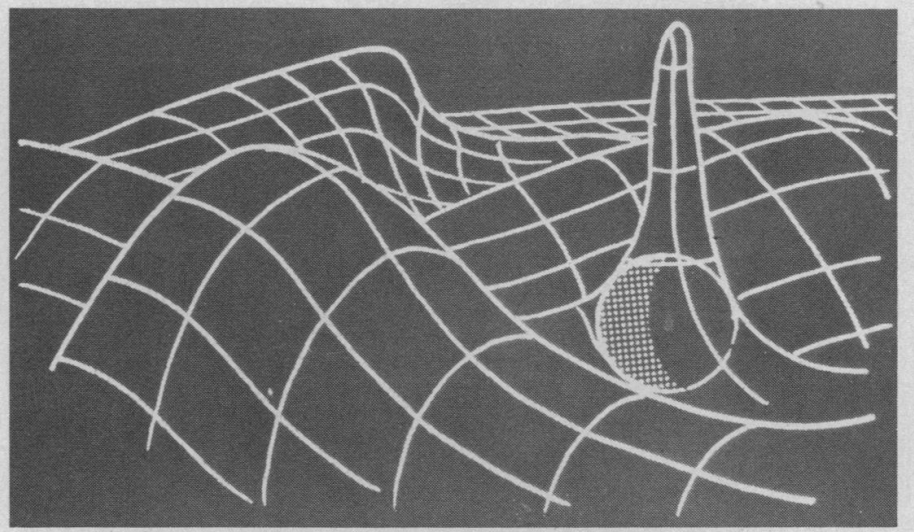
\includegraphics[width=0.3\linewidth]{bilder/rolling-ball.png} }}
    \caption{Visualization of a 2D and a 3D structuring element of a rolling ball algorithm.}
    \label{fig:rolling-ball}
\end{figure}